% =====================================================================
\chapter{System Design}
\label{ch:design}

\section{Architectural Overview}
\label{sec:design-arch}
\system{} follows a three-tier, event-driven architecture with four
cooperating components: a passenger mobile application, a web-based
administration console, a central application server, and a vehicle
GPS-acquisition layer. Two communication styles are used side by side,
each where it fits: stateless REST over HTTPS for command and query
operations (log in, fetch schedules, manage routes), and a persistent
WebSocket channel for the one thing that genuinely needs push semantics
---the live vehicle state. Figure~\ref{fig:arch} shows the complete
architecture.

\begin{figure}[H]
\centering
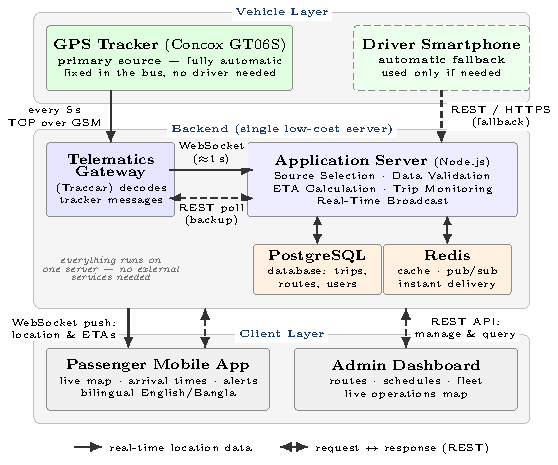
\includegraphics[page=1, width=0.9\textwidth]{twofigs.pdf}
\caption[System architecture of \system{}]{System architecture of
\system{}. The GPS tracker is the primary, fully automatic source; the
driver's smartphone is only a fallback. All backend components share one
low-cost server. Solid arrows carry real-time location data; dashed
double-headed arrows are REST request/response paths.}
\label{fig:arch}
\end{figure}

Three design decisions define the architecture:

\begin{enumerate}
  \item \textbf{Hardware-first acquisition.} The primary position source
  is a fixed, vehicle-grade tracker that operates with no human
  involvement. Anything a person must remember to do daily will
  eventually not be done; the design removes that failure mode entirely,
  and demotes the smartphone to an optional fallback
  (Section~\ref{sec:design-acquisition}).
  \item \textbf{A single low-cost server.} The application server,
  telematics gateway, database, and cache are co-hosted on one virtual
  private server. This satisfies NFR-3 and simplifies operations, while
  the Redis pub/sub back-plane preserves the option of scaling the
  realtime tier horizontally later (Section~\ref{sec:design-realtime}).
  \item \textbf{Event-driven processing.} Each arriving fix triggers a
  processing chain---arbitrate, filter, estimate, persist, publish---and
  everything downstream of the fix is pushed, never polled, so passenger
  latency is bounded by acquisition rather than by client refresh cycles.
\end{enumerate}

\section{Real-Time Data Flow}
\label{sec:design-flow}
Figure~\ref{fig:flow} traces the life of a single position report through
the system, grouped into three phases: acquisition (capture and
transmission), processing (arbitration, filtering, ETA computation), and
delivery (persistence, publication, and push). The seven steps of the
figure correspond to the design sections of this chapter and the
implementation sections of Chapter~\ref{ch:implementation}.

\begin{figure}[H]
\centering
\includegraphics[page=2, width=0.72\textwidth]{twofigs.pdf}
\caption[Real-time data flow]{Real-time data flow: the life of one
position report, from the GPS fix on the bus to the passenger's screen.
The timeline on the right shows representative latencies measured in the
pilot; the median end-to-end acquisition latency was 5.9\,s.}
\label{fig:flow}
\end{figure}

\section{GPS-Acquisition Layer}
\label{sec:design-acquisition}

\subsection{Primary Source: Fixed Vehicle Tracker}
The primary source is a Concox GT06S, a vehicle-grade GPS/GSM tracker
hard-wired to the bus's electrical system. While the vehicle moves, the
unit obtains a satellite fix every 5 seconds and transmits it over the
cellular network (TCP over GSM) to a self-hosted Traccar telematics
server, which implements the tracker's binary protocol and decodes each
message within about a second. Because the tracker is fixed to the
vehicle and powered from it, tracking requires no driver action, no
driver-owned device, and no driver data plan---the property on which the
whole operational-feasibility argument rests.

\subsection{Secondary Source: Driver Smartphone (Optional)}
A bus without a working tracker---not yet fitted, faulty, or SIM
depleted---can still be tracked. A driver smartphone running the app in
driver mode publishes its location to an authenticated REST endpoint.
This path is deliberately \emph{optional}: it exists so that coverage
degrades gracefully, not because the system depends on it. During the
pilot, two of the three buses were not yet fitted with trackers, so this
fallback path carried a substantial share of real trips
(Section~\ref{sec:eval-sources}).

\subsection{Ingesting from the Telematics Gateway}
The application server consumes Traccar's decoded positions through two
complementary paths, designed so that the faster one is used whenever
possible and the slower one guarantees delivery:

\begin{itemize}
  \item \textbf{Push (preferred).} A session-cookie WebSocket
  subscription to Traccar delivers each new fix within about one second
  of decoding.
  \item \textbf{Poll (backup).} A REST polling job queries Traccar every
  8 seconds during active trips, covering intervals when the socket is
  unavailable. (After the idle-efficiency optimization of
  Section~\ref{sec:eval-efficiency}, polling drops to every 60 seconds
  for buses with no active or imminent trip.)
\end{itemize}

\section{Source Arbitration Design}
\label{sec:design-arbitration}
When both a tracker and a driver phone are reporting for the same bus,
exactly one of them must drive the position passengers see. The design
maintains, per bus, one \emph{source-tracking state} for each active
source and a single \emph{canonical tracking state} for the public
position. On every inbound fix, an arbitration routine scores each
source's health---essentially its recency and validity---and selects the
canonical source by health and a configurable priority rank that prefers
the hardware tracker. Because the decision is re-evaluated per fix, a bus
can hand over from tracker to phone (or back) in the middle of a trip
with no passenger-visible artefact: the canonical marker simply continues
from the freshest healthy source. This satisfies FR-3 and NFR-2.

\section{Location-Quality Filtering Design}
\label{sec:design-filter}
Raw GPS cannot be displayed as-is. The design places a filtering pipeline
between arbitration and everything downstream, so that only credible
fixes can move the canonical position. Four operator-configurable rules
gate each fix:

\begin{enumerate}
  \item \textbf{Accuracy gate.} Fixes reporting accuracy worse than
  120\,m are soft-rejected; worse than 250\,m, hard-rejected.
  \item \textbf{Teleport guard.} A fix implying an inter-fix speed above
  120\,km/h is physically implausible on the pilot routes and is
  rejected.
  \item \textbf{Minimum-movement floor.} Displacements under 4\,m are
  treated as stationary, suppressing the GPS jitter that would otherwise
  make a parked bus wander on the map.
  \item \textbf{Freeze/release hysteresis.} Under sustained poor
  accuracy the marker is held still, and motion resumes only on a
  confident displacement, preventing oscillation at the accuracy
  boundary.
\end{enumerate}

The thresholds are deliberately conservative: 120\,km/h exceeds any
plausible bus speed on the pilot routes, and the 4\,m floor sits above
the tracker's typical urban scatter, so legitimate motion is never
suppressed. A short-window rolling average of accepted speeds is
maintained per trip and feeds the ETA estimator. Full HMM map matching
(Section~\ref{sec:lit-gps}) was considered and rejected: the buses follow
a small set of fixed routes, so projecting onto the known polyline
achieves the needed stability at a fraction of the cost.

\section{Arrival-Time Estimation Design}
\label{sec:design-eta}
The ETA estimator is geometric and training-free, chosen so the system
is fully functional from its first day of deployment
(Section~\ref{sec:lit-eta} explains why data-driven models were not an
option at cold start).

The route is first reduced to a cumulative along-path distance array over
its ordered stops. Each accepted fix is projected onto the nearest route
segment using a planar (local equirectangular) projection, which yields
the bus's \emph{progress} distance along the route and its cross-track
offset; the projection makes the estimate robust to lateral GPS error and
to the bus running slightly off the idealized polyline. For every stop
still ahead, the remaining distance is the difference between the stop's
cumulative distance and the bus's progress; dividing by an effective
speed yields that stop's ETA. The effective speed is the per-trip
rolling average when it is reliable ($\geq 5$\,km/h), otherwise a
configurable default of 20\,km/h. Each estimate carries a
\textsc{high}/\textsc{medium}/\textsc{low} confidence label derived from
the quality of the speed signal, so the interface can be honest about
uncertainty. A stop is marked \emph{reached} when the bus enters an
80\,m arrival radius, which triggers a stop-arrival event and, for
subscribed riders, a push notification (FR-9). The complete procedure is
given as Algorithm~\ref{alg:eta}.

\begin{algorithm}[H]
\caption{Estimating the ETA to every upcoming stop}
\label{alg:eta}
\begin{algorithmic}[1]
\Require current bus GPS fix; ordered route stops; recent average speed
\Ensure an ETA and a confidence label for each stop ahead
\State Compute each stop's distance from the route start (cumulative)
\State Project the bus fix onto the nearest route segment to find how far
  along the route it has travelled (its \emph{progress})
\If{recent average speed $\geq 5$\,km/h}
  \State $speed \gets$ recent average speed
\Else
  \State $speed \gets 20$\,km/h \Comment{fallback default}
\EndIf
\ForAll{stops ahead of the bus}
  \State $remaining \gets (\text{stop's distance}) - (\text{progress})$
  \State $\text{ETA} \gets remaining / speed$
\EndFor
\State Assign a confidence (High/Medium/Low) from the speed quality
\If{the nearest stop is within 80\,m}
  \State mark it reached and notify subscribed riders
\EndIf
\State \Return the ETA and confidence for every stop ahead
\end{algorithmic}
\end{algorithm}

\section{Trip Lifecycle Design}
\label{sec:design-lifecycle}
A trip is modelled as a state machine, shown in
Figure~\ref{fig:lifecycle}:
\textsc{planned} $\rightarrow$ \textsc{pre\_trip} $\rightarrow$
\textsc{running} $\rightarrow$ \textsc{ended}.

\begin{figure}[H]
\centering
\resizebox{\textwidth}{!}{%
\begin{tikzpicture}[font=\small, node distance=1.75cm,
  st/.style={draw, rounded corners=3pt, fill=blue!6, minimum width=2.5cm,
             minimum height=9mm, align=center},
  ar/.style={-{Latex[length=2.4mm,width=2mm]}, semithick}]
\node[st] (pl) {\textsc{planned}};
\node[st, right=of pl] (pt) {\textsc{pre\_trip}};
\node[st, right=of pt] (ru) {\textsc{running}};
\node[st, right=of ru] (en) {\textsc{ended}};
\draw[ar] (pl) -- (pt) node[midway, above, font=\footnotesize, align=center]
  {scheduled job\\opens window};
\draw[ar] (pt) -- (ru) node[midway, above, font=\footnotesize, align=center]
  {dwell inside\\origin geofence};
\draw[ar] (ru) -- (en) node[midway, above, font=\footnotesize, align=center]
  {trip completed\\or closed};
\node[below=4.5mm of pt, font=\footnotesize, text=black!60, align=center]
  {rider sees pre-departure state:\\parked / approaching / arrived at origin};
\node[below=4.5mm of ru, font=\footnotesize, text=black!60, align=center]
  {live tracking, ETAs,\\staleness monitoring};
\end{tikzpicture}}%
\caption{The trip lifecycle state machine. The \textsc{pre\_trip} state is
what keeps the passenger's map informative before departure.}
\label{fig:lifecycle}
\end{figure}

The distinctive state is
\textsc{pre\_trip}: a scheduled job opens a window before the scheduled
departure during which the rider sees the bus's pre-departure state
---parked, approaching the origin, or arrived at the origin---instead of
a blank map (FR-7). The vehicle auto-promotes to \textsc{running} when it
dwells inside the origin geofence. A staleness job runs every 30 seconds
and flags any trip whose latest fix has aged beyond a threshold, so a
frozen marker is presented as \emph{stale} rather than silently passed
off as live (FR-8). Honesty about data age is treated as a first-class
interface requirement, not an afterthought.

\section{Database Design}
\label{sec:design-database}
PostgreSQL is the system of record, accessed through the Prisma ORM. The
schema comprises 31 relational models organized into six functional
domains, shown in Figure~\ref{fig:schema}.

\begin{figure}[H]
\centering
\begin{tikzpicture}[font=\small,
  dom/.style={draw, rounded corners, fill=blue!6, align=left,
              text width=0.40\textwidth, inner sep=5pt, minimum height=11mm}]
  \node[dom] (a) {\textbf{Identity \& Auth}\\User, Session, Role, OTP};
  \node[dom, right=5mm of a] (b) {\textbf{Fleet \& Devices}\\Bus, GpsDevice, Assignment};
  \node[dom, below=5mm of a] (c) {\textbf{Routing \& Schedule}\\Route, Stop, RouteStop, Schedule};
  \node[dom, right=5mm of c] (d) {\textbf{Trip \& Tracking}\\Trip, LocationLog, TrackingState};
  \node[dom, below=5mm of c] (e) {\textbf{Comms \& Passenger}\\Notification, Favorite, Occupancy};
  \node[dom, right=5mm of e] (f) {\textbf{Audit \& Ops}\\AuditLog, TripEvent, IngestLog};
\end{tikzpicture}
\caption{The 31-model relational schema, grouped into six functional
domains (representative models shown for each domain).}
\label{fig:schema}
\end{figure}

Two domains matter most to the thesis argument. \emph{Trip \& Tracking}
separates the per-source tracking states from the canonical tracking
state, which is what makes the arbitration design of
Section~\ref{sec:design-arbitration} expressible in data. \emph{Audit \&
Ops} preserves every raw ingest and trip event; this is the layer that
made the retrospective analysis of Chapter~\ref{ch:evaluation}---
including the discovery of the 98\% idle-reporting waste---possible
without any additional instrumentation.

\section{Realtime Delivery Design}
\label{sec:design-realtime}
Realtime delivery uses Socket.IO over WebSocket. Each active trip is a
logical \emph{room}; a passenger tracking a trip joins that trip's room
and thereafter receives only that trip's events, bounding per-client
traffic to the single vehicle being observed. Redis serves as the
publish/subscribe back-plane: accepted canonical updates and recomputed
ETAs are published once, and every server process holding subscribers for
that trip forwards them. This lets the realtime tier scale horizontally
without losing fan-out consistency (NFR-6), even though the pilot ran
comfortably on a single process. Authentication is enforced both at
socket connection and at room join (NFR-5).

Offline behaviour is part of the same design: the client retains the most
recent state, so a transient disconnection degrades to a ``last known''
view with an explicit staleness indicator rather than an empty screen.

\section{Security Design}
\label{sec:design-security}
All client--server traffic runs over HTTPS. Passengers and administrators
authenticate against the identity domain of the schema; role-based
authorization separates passenger, driver, and administrator
capabilities. The driver-side location endpoint accepts reports only from
an authenticated driver bound to the bus in question, preventing
arbitrary clients from injecting positions. Socket connections carry the
same identity, and room joins are authorized per trip. Administrative
actions are recorded in the audit domain.

\section{Summary}
This chapter presented the three-tier, event-driven architecture of
\system{} and the design of each major component: dual-source GPS
acquisition with per-fix health arbitration, the four-gate
location-quality filter, the training-free geometric per-stop ETA
estimator, the trip lifecycle with its pre-trip and staleness states,
the 31-model relational schema, the room-based realtime delivery layer,
and the security model. Chapter~\ref{ch:implementation} describes how
each design was realized.
